
\section{Einordnung und weitere Visualisierung der Daten}
Im folgenden wird die Korrelation der Corona-Fälle der einzelnen deutschen Landkreise untersucht. Um dieses Verfahren besser zu verstehen und ein grobes Gefühl für den Datensatz zu bekommen, werden die einzelnen Werte gesondert an.

\subsection{Die deutschen Landkreise und Ihre Bevölkerungsdichte}
Zuallererst folgen die genutzten Daten, welche nichts mit Corona zutun haben: Die Landkreise und ihre Bevölkerungsdichte. Die Bevölkerungsdichte wird aus der Bevölkerungszahl und der Fläche des Landkreises berechnet, welche von der API bereitgestellt werden \todo{adäquate Verlinkung auf API}.

In Abbildung \autoref{fig:distribution_pop_density_counties} sind die Bevölkerungsdichten der einzelnen Landkreise dargestellt. Auf der linken Seite befindet sich die Verteilung und auf der rechten Seite die räumliche Anordnung.
Die Bezirke Berlins sind einzeln gelistet, daher entsprechen die sechs höchsten Bevölkerungsdichten den Berliner Bezirken  Friedrichshain-Kreuzberg, Mitte, Neukölln, Tempelhof-Schöneberg, Lichtenberg, Charlottenburg-Wilmersdorf, obwohl die Bevölkerungsdichte des gesamten Berliner Stadtkreises niedriger ist als die Bevölkerungsdichte Münchens (in dieser Auflistung Platz 7, ohne Berliner Bezirke Platz 1).

\begin{figure}[H]
    \centering
    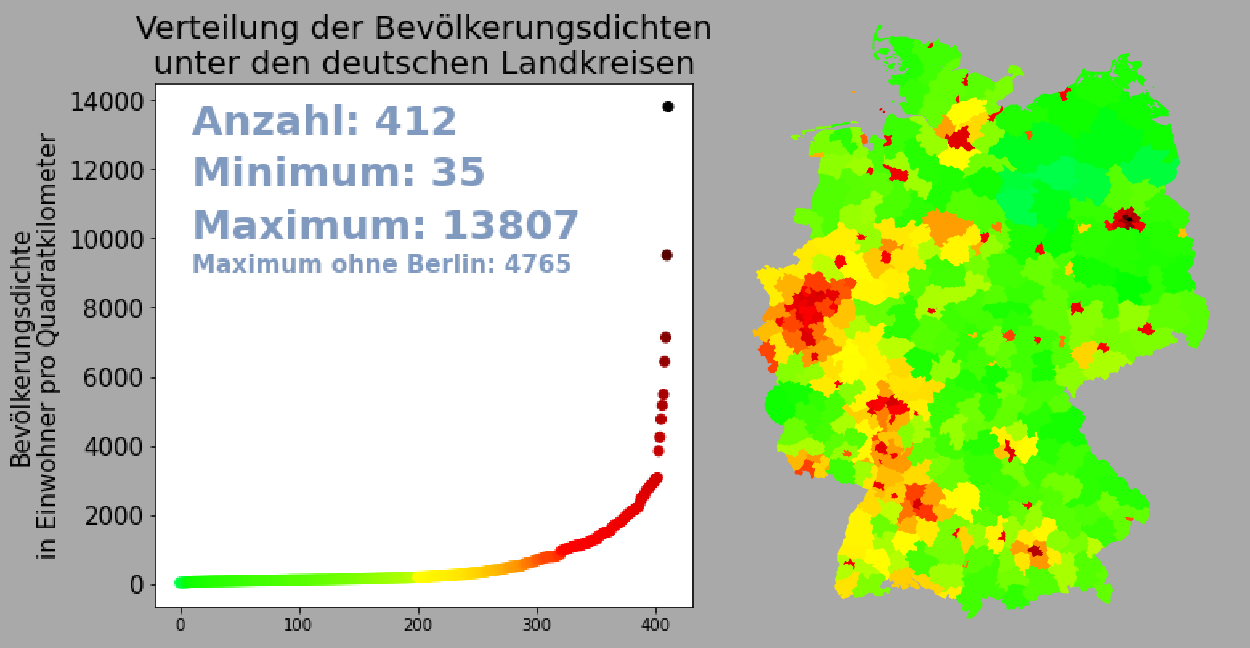
\includegraphics[width = 0.95\textwidth]{figures/Durchführung/population_density_counties_Distribution_and_map.png}
    \caption{Verteilung der Bevölkerungsdichten unter den deutschen Landkreisen.}
    \label{fig:distribution_pop_density_counties}
\end{figure}

\todo{klarstellen, das die Landkreise nicht den Landkreisen entsprechen (Berlin ist aufgeteilt) Aus Wikipedia "Landkreis": In Deutschland gibt es 294 Landkreise. Zusammen mit den 106 kreisfreien Städten bilden sie die insgesamt 400 Gebietskörperschaften auf Kreisebene. Wir haben 412.}
In Abbildung 


Teilt man die Landkreise nach den ersten beiden Kennzahlen des Landkreises, die des Bundeslandes und die des aktuellen (teils auch vergangenen) Regierungsbezirks, ein, ergibt sich für die Bevölkerungsdichte das in \autoref{fig:distribution_pop_density_districts} dargestellte Bild.

Nicht alle Bundesländer wurden in Regierungsbezirke unterteilt, in diesem Fall wird die Bevölkerungsdichte des Landkreises gewählt. Im folgenden wird dennoch von \glqq{}den Regierungsbezirken\grqq{} gesprochen. Zudem sind die Stadtstaaten Bremen und Hamburg zum Regierungsbezirk Lüneburg hinzugefügt und der Stadtstaat Berlin zum Bundesland Brandenburg hinzugefügt.

\begin{figure}[H]
    \centering
    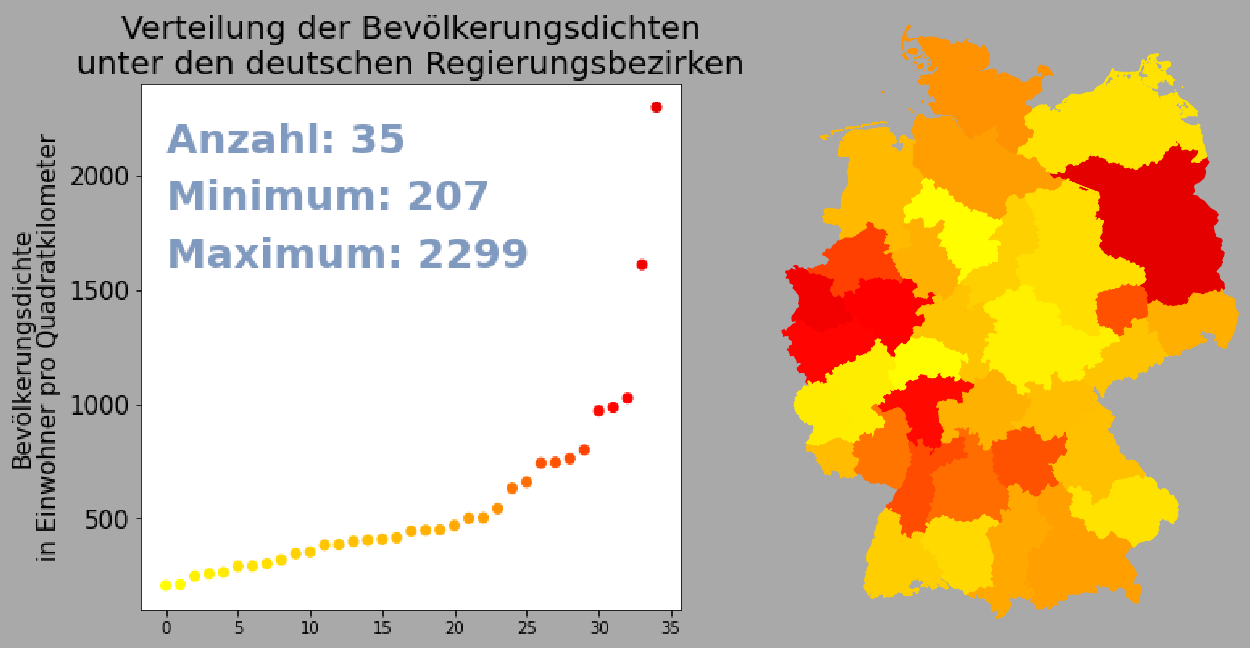
\includegraphics[width = 0.95\textwidth]{figures/Durchführung/population_density_districts_Distribution_and_map.png}
    \caption{Verteilung der Bevölkerungsdichten unter den deutschen Regierungsbezirken. Die Skalierung entspricht der Farbgebung in \autoref{fig:distribution_pop_density_counties}.}
    \label{fig:distribution_pop_density_districts}
\end{figure}

Klar zu erkennen sind die Stadtkreise in Abbildung \ref{fig:distribution_pop_density_counties}: Sie weisen eine hohe Bevölkerungsdichte auf und sind in der Regel von weniger stark bevölkerten Landkreisen umgeben.

Als erstes Beispiel zu Demonstrationszwecken ausführlich gezeigt.

Die Städte in Tabelle \ref{tab:landkreise_um_städte} von einem Landkreis umgeben, an Ihnen lässt sich besonders gut testen, ob sich in den Korrelationswahrscheinlichkeiten zwischen einer Stadt und ihrem Umland eine zeitliche Verschiebung feststellen lässt.
\begin{table}[H]
    \centering
    \begin{tabular}{c|c|c|c}
    Name des Land-&AGS &Umgebener  &AGS\\
    kreises (LK)  &Landkreis&Stadtkreis (SK)&Stadtkreis\\
    \hline
Kassel & 6633 & Kassel & 6611 \\\hdashline
Trier-Saarburg & 7235 & Trier & 7211 \\\hdashline
Südliche Weinstraße & 7337 & Landau i.d.Pfalz & 7313 \\\hdashline
Südwestpfalz & 7340 & Pirmasens & 7317 \\\hdashline
Heilbronn & 8125 & Heilbronn & 8121 \\\hdashline
Rastatt & 8216 & Baden-Baden & 8211 \\\hdashline
Rosenheim & 9187 & Rosenheim & 9163 \\\hdashline
Landshut & 9274 & Landshut & 9261 \\\hdashline
Straubing-Bogen & 9278 & Straubing & 9263 \\\hdashline
Amberg-Sulzbach & 9371 & Amberg & 9361 \\\hdashline
Neustadt a.d.Waldnaab & 9374 & Weiden i.d.OPf & 9363 \\\hdashline
Regensburg & 9375 & Regensburg & 9362 \\\hdashline
Bamberg & 9471 & Bamberg & 9461 \\\hdashline
\begin{comment}
Bayreuth & 9472 &  &  \\\hdashline
Coburg & 9473 &  &  \\\hdashline
Hof & 9475 &  &  \\\hdashline
Ansbach & 9571 &  &  \\\hdashline
Schweinfurt & 9678 &  &  \\\hdashline
Würzburg & 9679 &  &  \\\hdashline
Ostallgäu & 9777 &  &  \\\hdashline
\end{comment}
Oberallgäu & 9780 & Kempten & 9763 \\\hdashline
Potsdam-Mittelmark & 12069 & Brandenburg a.d. Havel & 12051 \\\hdashline
Spree-Neiße & 12071 & Cottbus & 12052 \\\hdashline
Saalekreis & 15088 & Halle (Saale) & 15002 \\\hdashline
Weimarer Land & 16071 & Weimar & 16055
    \end{tabular}
    \caption{Landkreise mit Name und Gemeindeschlüssel (AGS), die den jeweils mit Name und Gemeindeschlüssel gekennzeichneten Stadtkreis komplett umgeben.}
    \label{tab:landkreise_um_städte}
\end{table}

In Abbildung \autoref{fig:selected_counties} sind die ausgewählten Landkreise mit den Stadtkreisen, die sie umgeben abbgebildet.
\begin{figure}
    \centering
    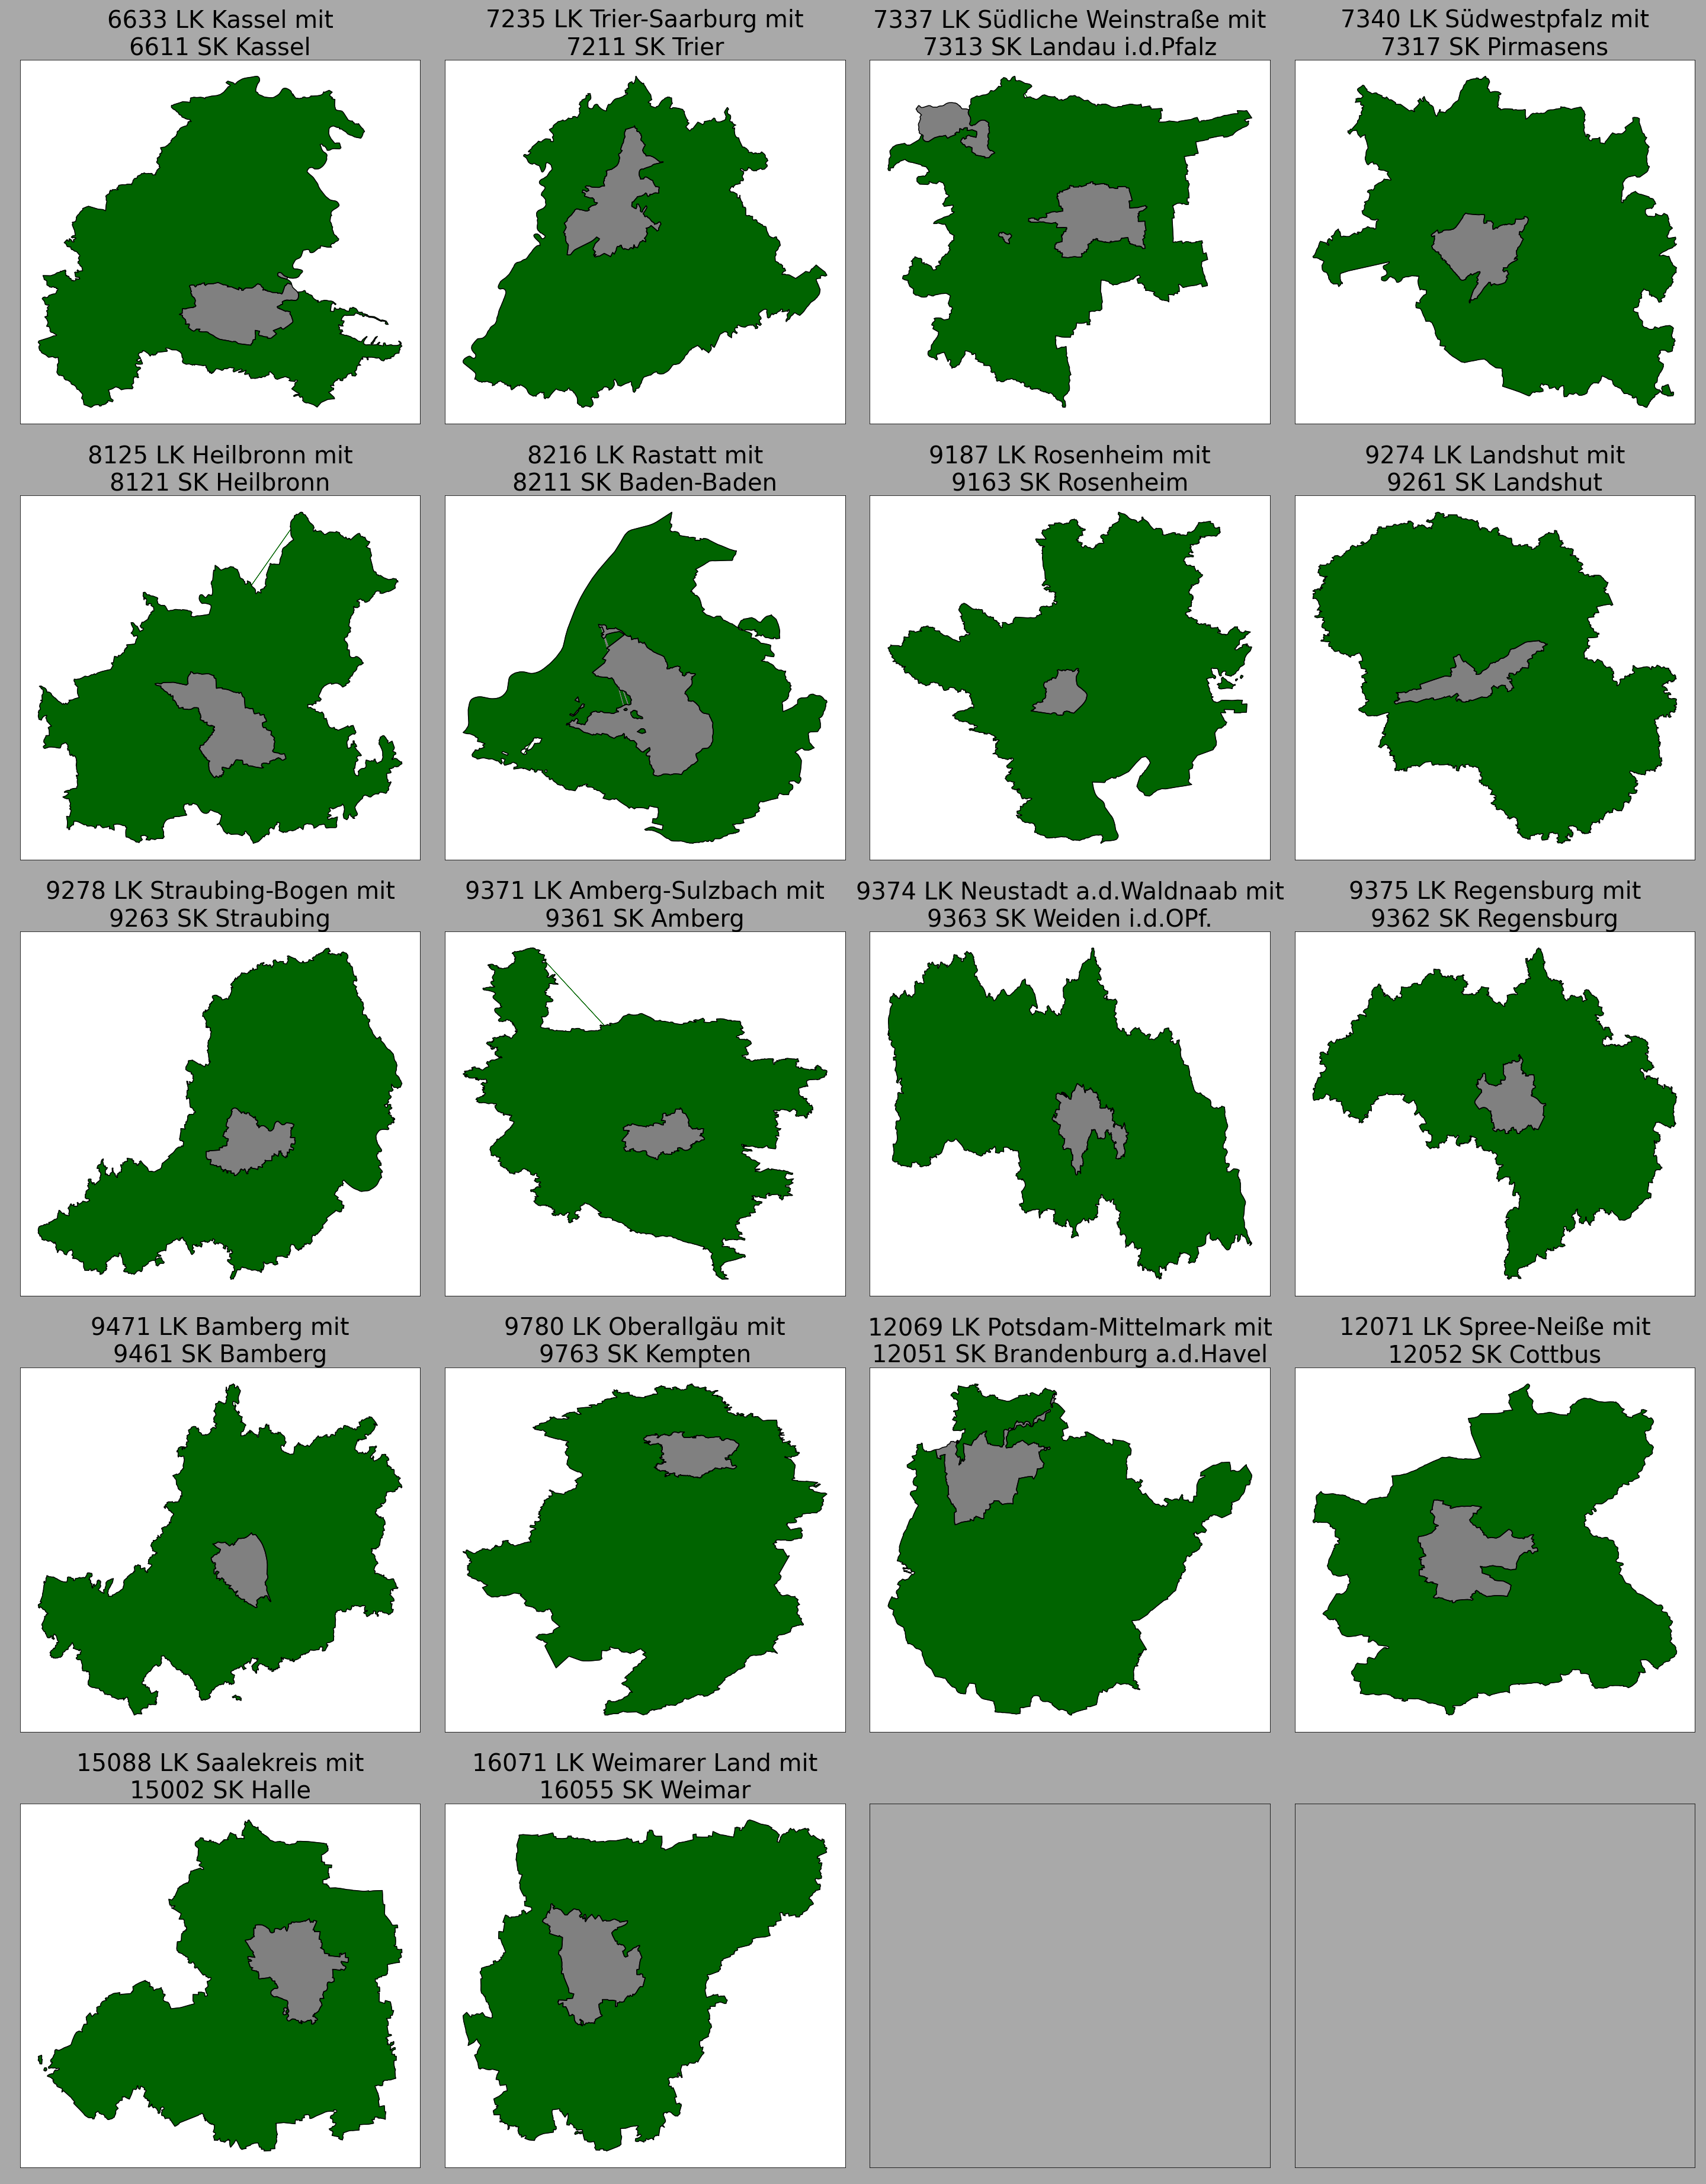
\includegraphics[width=\textwidth]{figures/Durchführung/selected_counties.png}
    \caption{Die ausgewählten Landkreise mit den Stadtkreisen, die sie jeweils umgeben.}
    \label{fig:selected_counties}
\end{figure}